\documentclass[11pt, letterpaper]{article}

% Packages
\usepackage[margin=0.85in]{geometry}
\usepackage{booktabs, tabularx, float}
\usepackage{enumitem}
\usepackage{parskip}
\usepackage{tikz}
\usetikzlibrary{arrows.meta, positioning, fit, backgrounds}
\usepackage{listings}
\usepackage{hyperref}

% Compact lists
\setlist{noitemsep, topsep=3pt, leftmargin=1.5em}

% Code listing style
\lstset{basicstyle=\ttfamily\footnotesize, breaklines=true, frame=single, xleftmargin=1em}

% Table row padding
\renewcommand{\arraystretch}{1.15}

% ── Title ─────────────────────────────────────────────────────
\title{%
    {\LARGE\bfseries ITCS5010 GenAI: NotebookLM Clone}\\[0.3em]
    {\large NotebookLM Clone Initial Plan}
}

\author{%
    \begin{tabular}[t]{ccc}
        Varad Paradkar & Nidhi Shah & Brinda Chinnaraji \\[0.3em]
        \multicolumn{3}{c}{Sai Kiran Jagini \quad Shar Adhiambo}
    \end{tabular}%
}

\date{February 19, 2026}

\begin{document}
\maketitle

% ──────────────────────────────────────────────────────────────
\section{System Overview}

\textbf{StudyPod} is a full-stack AI application modeled after Google's NotebookLM.
Authenticated users can:

\begin{enumerate}
    \item \textbf{Upload} documents (PDF, PPTX, TXT) or paste web URLs.
    \item \textbf{Chat} with their documents via Retrieval-Augmented Generation (RAG), receiving answers with inline source citations.
    \item \textbf{Generate} study artifacts: summary reports, quizzes with answer keys, and podcast audio.
\end{enumerate}

Each user maintains multiple \emph{notebooks}---self-contained workspaces with their own sources, chat history, and artifacts.
All user data is strictly isolated.
The system is hosted on \textbf{Hugging Face Spaces} (free tier) with CI/CD from GitHub.

\subsection{Design Principles}

\begin{itemize}
    \item \textbf{Zero cost} --- every component is free-tier or runs locally; no paid subscriptions.
    \item \textbf{Minimal complexity} --- ${\sim}12$ Python files, filesystem storage, no external database.
    \item \textbf{MVP first} --- core RAG chat ships before artifacts or advanced features.
    \item \textbf{Secure by default} --- per-user path isolation, server-side secrets, strict input validation.
\end{itemize}

% ──────────────────────────────────────────────────────────────
\section{Architecture \& Tool Stack}

\subsection{Technology Choices}

\begin{table}[H]
\centering\small
\begin{tabularx}{\textwidth}{@{}l l X@{}}
\toprule
\textbf{Layer} & \textbf{Tool} & \textbf{Rationale} \\
\midrule
Frontend   & Gradio                     & Python-only; built-in HF OAuth, chat, audio, and file-upload components \\
LLM        & Groq API (Llama 3.1 70B)   & Free tier (${\sim}$30 req/min); fast LPU inference; OpenAI-compatible SDK \\
Embeddings & sentence-transformers      & Runs locally on CPU; no API key; 384-dim vectors; ${\sim}$80 MB model \\
           & {\footnotesize(\texttt{all-MiniLM-L6-v2})} & \\
Vector DB  & ChromaDB (local)           & Free; file-based persistence; per-notebook collections \\
TTS        & edge-tts                   & Free; no API key; multiple high-quality voices \\
PDF        & PyMuPDF                    & Fast page-level text extraction \\
PPTX       & python-pptx                & Slide-by-slide text from all shapes \\
URLs       & trafilatura                & Strips ads/navigation; extracts main content \\
Chunking   & langchain-text-splitters   & \texttt{RecursiveCharacterTextSplitter}; 1000 chars, 200 overlap \\
Storage    & Local filesystem (\texttt{/data/}) & HF Spaces persistent directory; no external DB \\
Auth       & HF OAuth                   & Built-in via \texttt{gr.LoginButton()}; zero configuration \\
CI/CD      & GitHub Actions             & Auto-deploy to HF Space on push to \texttt{main} \\
\bottomrule
\end{tabularx}
\caption{Technology stack --- all components are free-tier or run locally.}
\end{table}

\subsection{Key Tradeoffs}

\textbf{Groq (Llama 3.1 70B) vs.\ OpenAI (GPT-4o-mini).}
Groq's free tier delivers ${\sim}$30 requests/min with sub-second latency via custom LPU hardware.
Llama 3.1 70B is competitive with GPT-4o-mini on RAG tasks.
Because Groq exposes an OpenAI-compatible endpoint, switching providers later requires only changing a \texttt{base\_url}.
The primary tradeoff is rate-limiting under heavy concurrent load, mitigated by retry logic and an 8B fallback model.

\textbf{Local Embeddings vs.\ Embedding API.}
Running \texttt{all-MiniLM-L6-v2} locally eliminates API costs and rate limits entirely.
The model produces 384-dimensional vectors in ${\sim}$50 ms per batch on CPU.
ChromaDB integrates with sentence-transformers natively.
The tradeoff is marginally lower embedding quality versus OpenAI's 1536-dim model---negligible for chunked-document retrieval.

\textbf{Filesystem vs.\ External Database.}
HF Spaces provides a persistent \texttt{/data} directory.
Storing everything on the filesystem (JSON, JSONL, raw files) avoids provisioning an external database.
The tradeoff: data is ephemeral on the free tier (lost after 48h of inactivity), which is acceptable per the assignment.

\subsection{Architecture Diagram}

\begin{figure}[H]
\centering
\resizebox{\textwidth}{!}{%
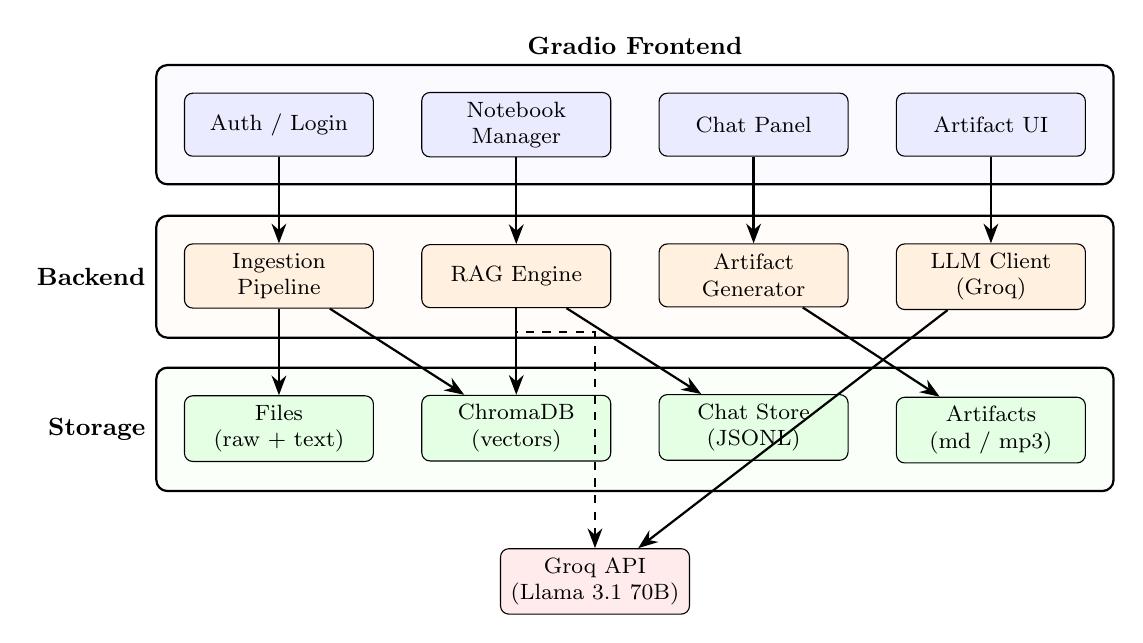
\begin{tikzpicture}[
    node distance=0.5cm and 0.6cm,
    box/.style={rectangle, draw, rounded corners=3pt, minimum width=2.4cm,
                minimum height=0.8cm, align=center, font=\footnotesize},
    arr/.style={-{Stealth[length=2.5mm]}, thick}
]
% Frontend row
\node[box, fill=blue!8] (auth)  {Auth / Login};
\node[box, fill=blue!8, right=of auth]  (nbmgr) {Notebook\\Manager};
\node[box, fill=blue!8, right=of nbmgr] (chat)  {Chat Panel};
\node[box, fill=blue!8, right=of chat]  (artui) {Artifact UI};

% Backend row
\node[box, fill=orange!12, below=1.1cm of auth]  (ingest) {Ingestion\\Pipeline};
\node[box, fill=orange!12, below=1.1cm of nbmgr] (rag)    {RAG Engine};
\node[box, fill=orange!12, below=1.1cm of chat]  (artgen) {Artifact\\Generator};
\node[box, fill=orange!12, below=1.1cm of artui] (llm)    {LLM Client\\(Groq)};

% Storage row
\node[box, fill=green!10, below=1.1cm of ingest] (files)  {Files\\(raw + text)};
\node[box, fill=green!10, below=1.1cm of rag]    (chroma) {ChromaDB\\(vectors)};
\node[box, fill=green!10, below=1.1cm of artgen] (chatst) {Chat Store\\(JSONL)};
\node[box, fill=green!10, below=1.1cm of llm]    (artst)  {Artifacts\\(md / mp3)};

% External
\node[box, fill=red!8, below=1.1cm of chroma, xshift=1cm] (groq) {Groq API\\(Llama 3.1 70B)};

% Grouped backgrounds
\begin{scope}[on background layer]
    \node[rectangle, draw, rounded corners=4pt, thick, fill=blue!2, inner sep=0.35cm,
          fit=(auth)(artui), label={[font=\small\bfseries]above:Gradio Frontend}] {};
    \node[rectangle, draw, rounded corners=4pt, thick, fill=orange!2, inner sep=0.35cm,
          fit=(ingest)(llm), label={[font=\small\bfseries]left:Backend}] {};
    \node[rectangle, draw, rounded corners=4pt, thick, fill=green!2, inner sep=0.35cm,
          fit=(files)(artst), label={[font=\small\bfseries]left:Storage}] {};
\end{scope}

% Frontend -> Backend
\draw[arr] (auth)  -- (ingest);
\draw[arr] (nbmgr) -- (rag);
\draw[arr] (chat)  -- (artgen);
\draw[arr] (artui) -- (llm);

% Backend -> Storage
\draw[arr] (ingest) -- (files);
\draw[arr] (ingest) -- (chroma);
\draw[arr] (rag)    -- (chroma);
\draw[arr] (rag)    -- (chatst);
\draw[arr] (artgen) -- (artst);

% Backend -> External
\draw[arr] (llm) -- (groq);
\draw[arr, dashed] (rag.south) -- ++(0,-0.3) -| (groq);
\end{tikzpicture}%
}
\caption{System architecture. The only external dependency is the Groq LLM API.}
\end{figure}

% ──────────────────────────────────────────────────────────────
\section{Component / Module Responsibilities}

The codebase is organized into four packages (${\sim}$12 files total):

\begin{table}[H]
\centering\small
\begin{tabularx}{\textwidth}{@{}l l X@{}}
\toprule
\textbf{Package} & \textbf{Module} & \textbf{Responsibility} \\
\midrule
\texttt{app.py}   & \emph{(entry point)} & Gradio layout, callback wiring, OAuth session management \\
\midrule
\texttt{core/}
    & \texttt{ingestion.py}   & Text extraction (PDF/PPTX/TXT/URL), chunking, embedding, ChromaDB upsert \\
    & \texttt{rag.py}         & Query embedding, top-$k$ retrieval, prompt construction, LLM call, citation parsing \\
    & \texttt{artifacts.py}   & Report / quiz / podcast generation; map-reduce for long sources; TTS \\
    & \texttt{llm\_client.py} & Groq API wrapper (OpenAI SDK); retry with exponential backoff \\
\midrule
\texttt{storage/}
    & \texttt{notebook\_store.py} & Notebook CRUD; \texttt{index.json}; directory lifecycle \\
    & \texttt{chat\_store.py}     & Append / read messages (JSONL) \\
    & \texttt{vector\_store.py}   & Per-notebook ChromaDB collection management \\
    & \texttt{artifact\_store.py} & Save / list / retrieve generated artifacts \\
\midrule
\texttt{utils/}
    & \texttt{config.py}     & Environment variables, model names, constants \\
    & \texttt{security.py}   & Path validation, filename sanitization, user-dir scoping \\
    & \texttt{extractors.py} & File-type--specific text extraction \\
\bottomrule
\end{tabularx}
\caption{Module responsibilities.}
\end{table}

% ──────────────────────────────────────────────────────────────
\section{Data Model \& Storage Strategy}

All data resides on the local filesystem under \texttt{/data/users/}. No external database is used.

\subsection{Directory Structure}

\begin{lstlisting}
/data/users/<username>/notebooks/
  |- index.json                       # notebook registry
  +- <notebook-uuid>/
       |- metadata.json               # name, sources, timestamps
       |- files_raw/                  # original uploads
       |- files_extracted/            # plain-text versions
       |- chroma/                     # ChromaDB persistent store
       |- chat/messages.jsonl         # chat history (one JSON/line)
       +- artifacts/
            |- reports/*.md
            |- quizzes/*.md
            +- podcasts/*.md + *.mp3
\end{lstlisting}

\subsection{Key Schemas}

\begin{itemize}
    \item \textbf{Notebook Index} (\texttt{index.json}) ---
          JSON array of notebooks, each with \texttt{id} (UUID), \texttt{name},
          \texttt{created\_at}, \texttt{updated\_at}, and \texttt{source\_count}.

    \item \textbf{Chat History} (\texttt{messages.jsonl}) ---
          One JSON object per line. User messages: \texttt{role}, \texttt{content}, \texttt{timestamp}.
          Assistant messages add \texttt{citations} (source file, chunk ID, page, excerpt),
          \texttt{rag\_technique}, and timing metrics.

    \item \textbf{ChromaDB Documents} ---
          Each chunk stores metadata: \texttt{source\_file}, \texttt{chunk\_index},
          \texttt{page\_number}, \texttt{char\_start/end}, \texttt{ingested\_at}.
\end{itemize}

\subsection{Storage Rationale}

\begin{itemize}
    \item \textbf{Filesystem over external DB} --- HF Spaces provides \texttt{/data}; avoids cost and complexity.
    \item \textbf{JSONL for chat} --- append-only writes; easy to stream-read; no migrations.
    \item \textbf{Per-notebook ChromaDB} --- full vector isolation; deleting a notebook = deleting a directory.
    \item \textbf{Atomic writes} --- metadata uses write-to-temp-then-rename to prevent corruption.
\end{itemize}

% ──────────────────────────────────────────────────────────────
\section{End-to-End Flows}

\subsection{Ingestion Pipeline}

\begin{enumerate}
    \item User uploads a file (PDF / PPTX / TXT) or enters a URL.
    \item System validates file type (whitelist) and enforces a 50 MB size limit.
    \item Raw file is saved to \texttt{files\_raw/}.
    \item Text is extracted via the appropriate library (PyMuPDF, python-pptx, or trafilatura).
    \item Extracted text is saved to \texttt{files\_extracted/}.
    \item Text is chunked with \texttt{RecursiveCharacterTextSplitter} (1000 chars, 200 overlap).
    \item Chunks are embedded locally via \texttt{all-MiniLM-L6-v2} (384-dim).
    \item Embeddings + metadata are upserted into the notebook's ChromaDB collection.
    \item Notebook metadata is updated (source count, timestamp).
\end{enumerate}

\subsection{RAG Chat with Citations}

\begin{enumerate}
    \item User types a question in the chat panel.
    \item The query is embedded with the same local model.
    \item ChromaDB returns the top-$k$ ($k{=}5$) chunks by cosine similarity.
    \item A prompt is assembled: system instructions (\emph{``answer only from context; cite sources''}), retrieved chunks with metadata, recent chat history, and the question.
    \item The prompt is streamed to Groq (Llama 3.1 70B).
    \item The response renders in the chat panel with inline citations (e.g., \texttt{[Source: lecture.pdf, p.3]}).
    \item Both messages are appended to \texttt{messages.jsonl}.
\end{enumerate}

\subsection{Artifact Generation}

\begin{enumerate}
    \item User clicks \textbf{Generate Report}, \textbf{Quiz}, or \textbf{Podcast}.
    \item All extracted texts from the notebook are gathered.
    \item If the combined text exceeds the context window, a \emph{map-reduce} strategy summarizes each source, then merges.
    \item An artifact-specific prompt is sent to the LLM:
          \begin{itemize}
              \item \textbf{Report} --- structured summary with headings and source refs.
              \item \textbf{Quiz} --- $N$ questions (MCQ / short-answer / T-F) + answer key.
              \item \textbf{Podcast} --- conversational transcript covering key topics.
          \end{itemize}
    \item Markdown output is saved to \texttt{artifacts/<type>/}.
    \item \emph{Podcast only:} transcript is synthesized to MP3 via edge-tts.
    \item The artifact appears in the UI with view / download / play controls.
\end{enumerate}

% ──────────────────────────────────────────────────────────────
\section{Security Plan}

\subsection{Authentication}

Users authenticate via \textbf{Hugging Face OAuth}, integrated through Gradio's \texttt{gr.LoginButton()}.
The OAuth flow is handled entirely by the HF platform; our app receives a verified username via \texttt{gr.OAuthProfile}. No passwords are stored.

\subsection{User Data Isolation}

\begin{table}[H]
\centering\small
\begin{tabularx}{\textwidth}{@{}l X@{}}
\toprule
\textbf{Threat} & \textbf{Mitigation} \\
\midrule
Path traversal &
    All paths are constructed from a sanitized \texttt{username} + UUID \texttt{notebook\_id}.
    A \texttt{validate\_path()} helper calls \texttt{Path.resolve()} and asserts the result is inside the user's directory. \\
\addlinespace
Cross-user access &
    Every backend call scopes to \texttt{/data/users/<username>/}. No raw paths are accepted from the client. \\
\addlinespace
Notebook ID guessing &
    IDs are UUID4 (128-bit random); brute-force enumeration is infeasible. \\
\addlinespace
Prompt injection &
    System prompt restricts the LLM to answering \emph{only} from provided context. User input is delimited with explicit markers. \\
\bottomrule
\end{tabularx}
\caption{Security threats and mitigations.}
\end{table}

\subsection{Secret Management}

Only \textbf{two secrets} are required:

\begin{table}[H]
\centering\small
\begin{tabularx}{\textwidth}{@{}l l X@{}}
\toprule
\textbf{Secret} & \textbf{Stored In} & \textbf{Scope} \\
\midrule
\texttt{GROQ\_API\_KEY} & HF Space Secret   & Server-side only; never exposed to the browser \\
\texttt{HF\_TOKEN}      & GitHub Repo Secret & CI/CD pipeline only \\
\bottomrule
\end{tabularx}
\caption{Complete secret inventory.}
\end{table}

\subsection{Input Validation}

\begin{itemize}
    \item \textbf{File uploads} --- extension whitelist (\texttt{.pdf}, \texttt{.pptx}, \texttt{.txt}); max 50 MB.
    \item \textbf{URLs} --- scheme whitelist (\texttt{http/https}); 30-second fetch timeout.
    \item \textbf{Notebook names} --- alphanumeric + spaces + hyphens; max 100 characters.
    \item \textbf{Filenames} --- strip \texttt{../}, \texttt{/}, \texttt{\textbackslash}, and null bytes.
\end{itemize}

% ──────────────────────────────────────────────────────────────
\section{Milestone Plan}

\subsection{Phase 1 --- MVP}

\begin{table}[H]
\centering\small
\begin{tabularx}{\textwidth}{@{}c X r@{}}
\toprule
\textbf{\#} & \textbf{Task} & \textbf{Effort} \\
\midrule
1 & Project scaffolding: repo, \texttt{requirements.txt}, GitHub Actions CI & 2h \\
2 & HF OAuth login / logout + session-state management & 2h \\
3 & Notebook CRUD (create, list, switch, delete) & 3h \\
4 & File upload + text extraction (PDF, TXT) & 3h \\
5 & Chunking + local embedding + ChromaDB storage & 2h \\
6 & Basic RAG chat (retrieve $\to$ prompt $\to$ respond) & 3h \\
7 & Chat-history persistence (JSONL) & 1h \\
8 & Deploy to Hugging Face Space & 1h \\
\midrule
  & \textbf{MVP total} & \textbf{17h} \\
\bottomrule
\end{tabularx}
\caption{Phase 1 --- Minimum Viable Product.}
\end{table}

\subsection{Phase 2 --- Core Features}

\begin{table}[H]
\centering\small
\begin{tabularx}{\textwidth}{@{}c X r@{}}
\toprule
\textbf{\#} & \textbf{Task} & \textbf{Effort} \\
\midrule
9  & PPTX and URL ingestion support & 2h \\
10 & Citation rendering in chat panel & 2h \\
11 & Report generation (\texttt{.md}) & 2h \\
12 & Quiz generation (\texttt{.md} with answer key) & 2h \\
13 & Podcast generation (transcript + TTS audio) & 3h \\
14 & Artifact listing, viewing, and download & 1h \\
\midrule
   & \textbf{Phase 2 total} & \textbf{12h} \\
\bottomrule
\end{tabularx}
\caption{Phase 2 --- Full feature set.}
\end{table}

\subsection{Phase 3 --- Polish \& Deliverables}

\begin{table}[H]
\centering\small
\begin{tabularx}{\textwidth}{@{}c X r@{}}
\toprule
\textbf{\#} & \textbf{Task} & \textbf{Effort} \\
\midrule
15 & RAG technique comparison (Naive vs.\ HyDE vs.\ Reranking) & 3h \\
16 & UI polish: error handling, loading states, responsive layout & 2h \\
17 & Documentation: architecture doc, README, RAG comparison & 2h \\
\midrule
   & \textbf{Phase 3 total} & \textbf{7h} \\
\bottomrule
\end{tabularx}
\caption{Phase 3 --- Polish and documentation.}
\end{table}

\subsection{Stretch Goals (If Time Permits)}

\begin{itemize}
    \item YouTube video transcript ingestion
    \item Selective file enable / disable for RAG queries
    \item Custom user prompt to focus artifact generation
    \item Two-speaker conversational podcast
\end{itemize}

% ──────────────────────────────────────────────────────────────
\section{Key Risks \& Mitigation}

\begin{table}[H]
\centering\small
\begin{tabularx}{\textwidth}{@{}X c c X@{}}
\toprule
\textbf{Risk} & \textbf{Impact} & \textbf{Prob.} & \textbf{Mitigation} \\
\midrule
Groq rate limits (30 req/min) & High & Med &
    Exponential-backoff retry; ``please wait'' UI; fallback to 8B model \\
\addlinespace
HF Space data loss on rebuild/sleep & Med & High &
    Acceptable per assignment; document limitation; \$5/mo paid tier if needed \\
\addlinespace
Large-file processing timeouts & Med & Med &
    50 MB upload cap; progress bar; batch processing \\
\addlinespace
Embedding model startup latency & Low & Med &
    Load once at startup (${\sim}$30s); keep in memory for session \\
\addlinespace
Scope creep & High & Med &
    Strict MVP-first; stretch goals only after core is stable \\
\addlinespace
Team coordination & Med & Med &
    Clear module ownership; feature branches; PR reviews \\
\bottomrule
\end{tabularx}
\caption{Risk register with impact, probability, and mitigation.}
\end{table}

% ──────────────────────────────────────────────────────────────
\section{RAG Techniques to Compare}

We will implement and benchmark four retrieval strategies:

\begin{table}[H]
\centering\small
\begin{tabularx}{\textwidth}{@{}l X X@{}}
\toprule
\textbf{Technique} & \textbf{How It Works} & \textbf{Tradeoff} \\
\midrule
Naive RAG &
    Embed query $\to$ cosine similarity $\to$ top-$k$ $\to$ prompt &
    Fast, simple; serves as baseline \\
\addlinespace
HyDE &
    LLM generates a hypothetical answer; embed \emph{that} to retrieve &
    Better recall for abstract Qs; +1 LLM call \\
\addlinespace
Reranking &
    Retrieve top-20 $\to$ cross-encoder rerank $\to$ top-5 &
    Higher precision; added latency \\
\addlinespace
Multi-Query &
    LLM generates 3 query variants $\to$ retrieve each $\to$ merge &
    Better recall for ambiguous Qs; 3$\times$ embed cost \\
\bottomrule
\end{tabularx}
\caption{RAG techniques planned for comparison.}
\end{table}

\textbf{Metrics:} retrieval relevance (manual eval), response quality, and end-to-end latency.

% ──────────────────────────────────────────────────────────────
\section{Specifications Written}

In addition to this design brief, we produced four specification documents (available in the repository under \texttt{docs/}):

\begin{itemize}
    \item \textbf{Component Specifications} (\texttt{component-specs.md}) ---
          function signatures, data classes, and interfaces for every backend module.
    \item \textbf{Data Model Specification} (\texttt{data-model-spec.md}) ---
          full JSON schemas, directory layout, ChromaDB metadata, data-lifecycle events.
    \item \textbf{UI \& Workflow Specification} (\texttt{ui-workflow-spec.md}) ---
          wireframe, user-journey flows, Gradio component mapping, callback wiring.
    \item \textbf{CI/CD Specification} (\texttt{ci-cd-spec.md}) ---
          GitHub Actions workflow, required secrets/variables, deployment flow.
\end{itemize}

\end{document}
